% !TEX root=template.tex

%Arquitetura: 

%Fazer descrição do sistema como um todo, incluir os diagramas já feitos. (MAS e ME) DONE

%Criar diagramas a explicar como o sistema em determinados use cases (durante desenvolvimento, manutenção, integração de novos agentes, etc) (ME) DONE

%TODO: Diagrama de componentes com os vários componentes do sistema e quem é que tem interfaces com quem (ME)

%TODO: Diagrama de atividades onde demonstras a evolução do sistema ao longo do tempo, para que o leitor perceba como este evolui, decisões, etc. (MAS e ME) (Sequence Diagrams)

%TODO: Descrever que o sistema foi desenhado tendo em conta a arquitetura com estes três agentes (RA, PA, TA) e que o RA e TA são os únicos que instanciam module engines. (MAS e ME)

%TODO: Explicar que os agentes utilizam o conceito de skill para que os RAs e TAs disponibilizem as suas capacidades e para que os PAs encontrem e peçam as capacidades que precisam. (MAS)

%TODO: Depois explicar como é que isto tudo funciona já com os agentes em causa. (MAS e ME) (Sequence Diagrams já feitos)



\typeout{NT FILE architecture.tex}

\glsresetall

\prependtographicspath{{Chapters/Figures/}}

\chapter{Architecture}
\label{cha:architecture}

In this section, the designed architecture for the proposed solution is explained. Starting with an overview of the system, the main architecture is presented, followed by a few usage scenarios. Then each component of the system is identified, how they work and how they are connected through the interfaces they use to communicate with other components. Normal system operations are overviewed and the supporting \acrlong{MAS} that was built to showcase the integration solution is explained. Every agent is presented in detail and a full system architecture is pictured at the end.

\section{System Architecture}
\label{sec:developed_architecture}

The main objective of this architecture is to bridge the gap between software and hardware. More specifically, to allow for a cyber-physical entity to interface with any kind of hardware in a flexible manner. To allow this flexibility, the system needs to be modular to an extent, enough to allow compatibility for many types of hardware, but not so much to make it hard to work with. A main entity must allow for the interfacing with the modular part of the interface, to enable support of multiple physical entities.\\ 

In addition, some supporting architecture is also needed to deploy the cyber-physical entities. This architecture must provide the main interface entity with a list of all integration modules available, so that it is able to load them.

These modules must then be supplied with the right configurations so that they are able to interface with the hardware. These configurations are also provided to the main entity by the supporting architecture, but are then sent to the modules.\\

The system proposed in this work then consists of two main components, a \acrfull{ME} and the \acrfullpl{LL}, with a deployment entity capable of providing these two components with the right resources. The \acrlong{ME} is the main entity that operates between the layers of software, in this case the agent, and hardware. It allows the agent to interface with any kind of hardware by loading \acrlongpl{LL}.\\

These \acrshortpl{LL} are what actually communicate to the hardware below, and must be able to use any kind of communication protocols. Due to their modularity, any \acrshort{LL} can be used at any point, independent of the characteristics of the agents above them. They are made with flexibility in mind to allow for the integration of any kind of hardware.\\

The \acrshort{ME} must be equally as flexible to allow for switching on the fly, during system operations. This allows for a more flexible and adaptable \acrshort{MAS}, since communications protocols can be switched fairly easy, the system becomes more robust also. To accomplish this, the \acrshortpl{LL} need to be loosely linked to the \acrshort{ME}.\\

As described previously the auxiliary architecture must provide the \acrshort{ME} with a list of all the available \acrshortpl{LL}. It must also provide the \acrshort{LL} with the correct configurations so that they can interface with the hardware. This could be done by passing all necessary resources to the agent on launch, and then the agent passes them along to the \acrshort{ME} and \acrshortpl{LL}. This support architecture can be a simple entity that, upon deploying the agents, supplies them with the correct resources that are in turn passed to the \acrshort{ME} and \acrshortpl{LL}. In this case, the deployment entity approach was chosen, but it would be possible to deploy an agent using the \acrshort{ME} through other means. As long as the \acrshort{ME} is supplied with the resources it needs to operate, it is able to perform its function. In Figure~\ref{fig:system_architecture}, the three main layers of our cyber-physical entity are shown, along with the deployment entity. There is an agent, which will take care of the decision making, the \acrshort{ME} and \acrshort{LL} which will provide an interface between agent and device, and the hardware itself, that will actuate on the physical world and provide sensor information to the agent above. It should matter not what kind of agent or hardware the agent is using, with the \acrlong{ME}, it must be capable of interfacing with it.

\begin{figure}[h!]
	\centering
	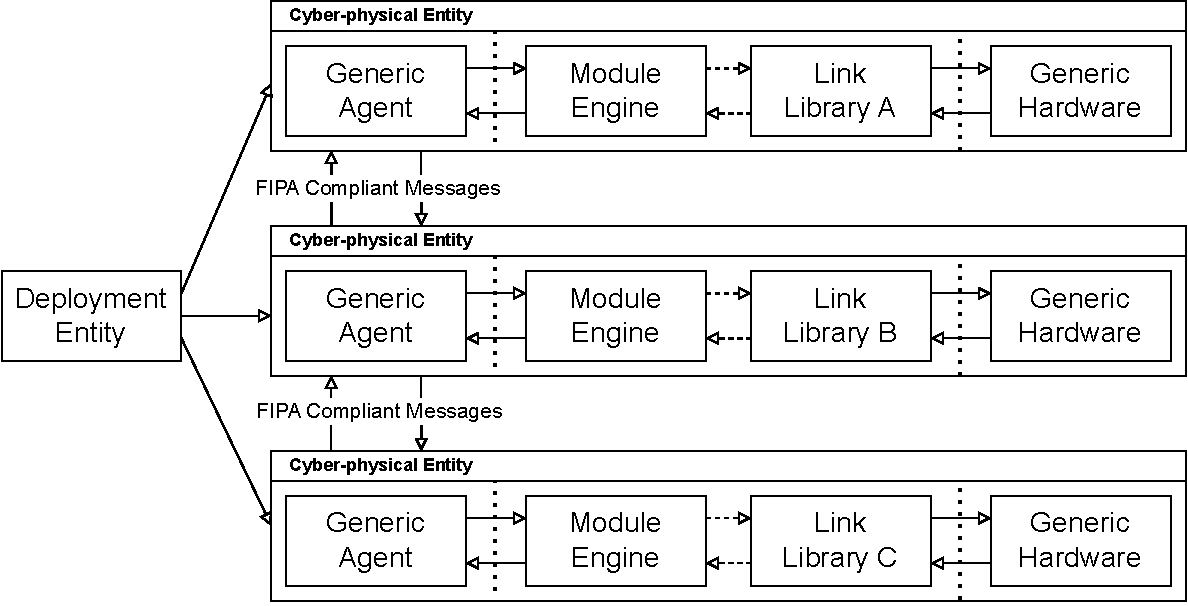
\includegraphics[scale=0.70]{System_Architecture}
	\caption{System architecture.}
	\label{fig:system_architecture}
\end{figure}

To summarize, the main objective of this project is to facilitate the integration of agents with their hardware, through the dynamic instantiation of \acrlongpl{LL} by the \acrlong{ME} and by allowing the \acrshortpl{LL} to be reused by many kinds of agents. This would also facilitate development of new \acrlongpl{LL}, since the architecture is prepared to work with new \acrshortpl{LL} from the get go.

\section{Usage Scenarios}
\label{sec:use_cases}

This system has three main usage scenarios. The first is when a developer is creating a new agent to add to either a new system or a previously existing one. The second is when a developer wants to create a new \acrshort{LL} to integrate a new type of hardware, or to use a different communications protocol. The third is when the already operating \acrshort{MAS} runs into an hardware problem, and needs to use other types of hardware to reduce system downtime. This scenario can also be applied when a new agent is integrated into the already operating \acrshort{MAS}, since it is in part what is happening when an agent needs replacement.\\

When a developer is creating a new agent, they need to make sure to use the \acrlong{ME} together with the agents that need to interface to the hardware. For obvious reasons, those agents that do not use hardware do not need the \acrshort{ME}. They also need to make sure that the \acrshort{LL} they wish to use to communicate with the hardware is already developed. If not, then they need to create it. The creation of new \acrlongpl{LL} will be explained in another scenario. 

The agent should be able to call the \acrshort{ME} at any point during its operation, whenever it need to instruct the hardware. It should also be able to retrieve the result of the operation from the hardware. Figure~\ref{fig:me_dev_use_case} shows a diagram representing this scenario. The development of the agent is unrelated to the hardware, since the \acrshort{ME} allows a more loose connection between the two. This is one of the advantages of the \acrlong{ME}. They can both be done in parallel to speed up development time.\\

To develop a new \acrlong{LL} a developer only needs to pick a new protocol and start development. As long as they respect the interfaces and methods for an \acrshort{LL}, better explained in Chapter~\ref{cha:implementation}, the \acrshort{ME} should be able to load it. In addition, the hardware also needs to implement the same communication protocol implemented by the \acrshort{LL}. If the hardware supports \acrshort{HTTP} requests, for instance, the \acrshort{LL} would need to implement a way to communicate through \acrshort{HTTP} requests. When development is complete, this new \acrshort{LL} can be published in some software distribution system, GitHub for instance, to be freely available to other developers wishing to use it. This scenario can be seen in Figure~\ref{fig:ll_dev_use_case}.

\begin{figure}[H]
	\centering
	\subbottom[New agent development scenario.\label{fig:me_dev_use_case}]{%
		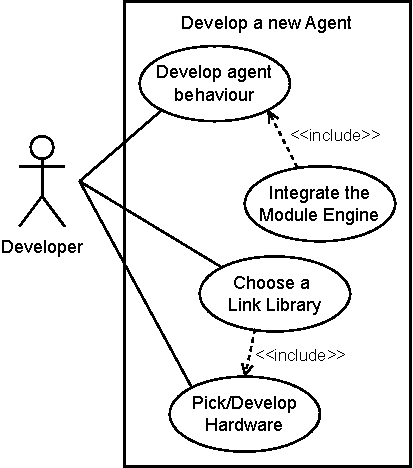
\includegraphics[width=0.45\linewidth]{ME_Dev_Use_Case}}%
	\hspace{0.50cm}
	\subbottom[New \acrlong{LL} development scenario.\label{fig:ll_dev_use_case}]{%
		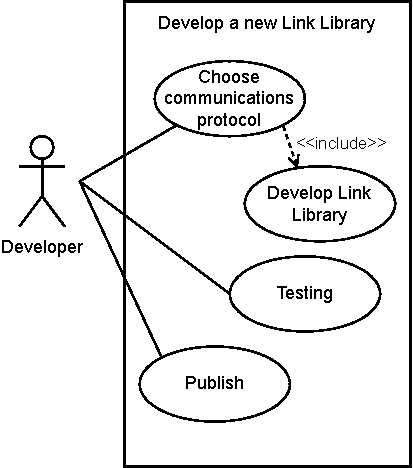
\includegraphics[width=0.45\linewidth]{LL_Dev_Use_Case}}%
	\caption{\acrlong{DA} activity diagram.}
	\label{fig:dev_use_case}
\end{figure}

Finally, performing maintenance on a system using the \acrshort{ME} reduces system downtime, since if and when there is a fault, new hardware can easily be integrated. The \acrlong{ME} should allow this, and since \acrlongpl{LL} are more flexible than traditional hardware integrations, they can be replaced easily by selecting a different \acrshort{LL} from the already available ones. If there is not an adequate \acrshort{LL}, a new one can be developed. Since they are relatively small, it might be faster to create a new \acrshort{LL} than to create a new traditional interface for the hardware. It also follows that integrating new agents into the pre-existing \acrshort{MAS} is as easy, since both processes share similarities, as shown in Figure~\ref{fig:agent_maintenance_use_case}.\\

\begin{figure}[h!]
	\centering
		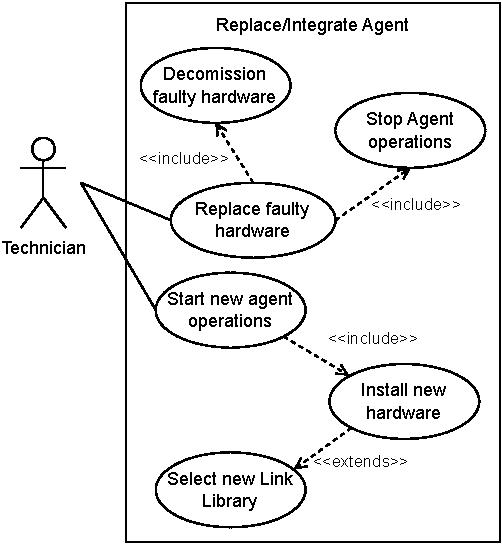
\includegraphics[scale=0.75]{Agent_Maintenance_Use_Case}
	\caption{Agent replacement/integration scenario.}
	\label{fig:agent_maintenance_use_case}
\end{figure}

\section{System Components}
\label{sec:system_components}

The developed system is to be inserted between agent and hardware layers to allow for a more flexible interface. The cyber-physical entity of which the agent is part of is composed of four main components. The agent itself, the \acrlong{ME} tasked with loading the \acrlongpl{LL}, the \acrshort{LL} capable of interfacing with the hardware, and the hardware represented by the agent. The agent, the \acrshort{ME} and the \acrshort{LL} can be considered the cyber part of the cyber-physical entity, with the hardware being the physical part.\\

In Figure~\ref{fig:component_diagram}, a Deployment Entity is also represented. This is the entity tasked with launching an agent using the \acrshort{ME} and also provide it with the initial parameters. Once again, this entity could be replaced with any other system, as long as the \acrshort{ME} receives its parameters, it should operate normally. These parameters allow the \acrshort{ME} to know what \acrlongpl{LL} exist, which one is to be used and also give the \acrshort{LL} its configurations needed to establish a connection to the hardware. Both the marketplace file and the \acrshort{LL} type are parameters used by the \acrshort{ME}, to load an \acrshort{LL}. The configurations need to be passed to the \acrlong{LL}, as they are \acrshort{LL} specific.\\

\begin{figure}[h!]
	\centering
	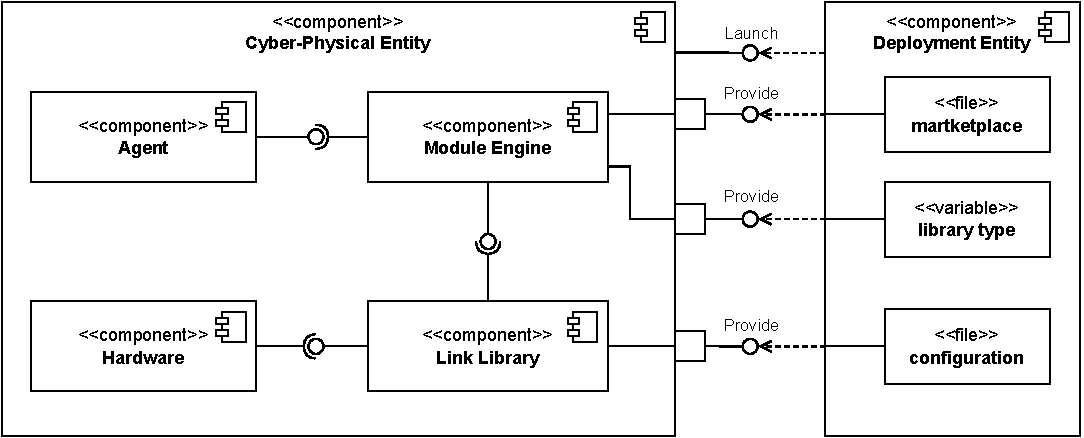
\includegraphics[scale=0.70]{Component_Diagram}
	\caption{Component diagram of a cyber-physical entity using the \acrlong{ME}.}
	\label{fig:component_diagram}
\end{figure}

Because the \acrlongpl{LL} are modular, these would need to be designed and implemented by other developers working with the \acrlong{ME}, wishing to create \acrshortpl{LL} with new protocols. To create a new one, a few specifications need to be followed in order to make sure the \acrshort{LL} is able to communicate with the \acrshort{ME} without problems. The \acrshort{LL} must establish the connection with the hardware upon being loaded, through the protocol it implements. It also must be able to close this connection at any point, since these \acrshortpl{LL} can be switched arbitrarily. Lastly, an \acrshort{LL} needs to be able to communicate to the hardware through the protocol it implements. This means that the hardware would also need to implement the same protocol in order to establish a connection. It would also be possible to develop an \acrshort{LL} capable of directly interfacing with the hardware through a more specific communication channel, by hosting the agent on the same device as the hardware, for instance. As long as a \acrlong{LL} implements it, it should be possible to use any communication channel. No information is exchanged exclusively between the loaded \acrlong{LL} and the \acrlong{ME}, which makes development easier, since no protocols need to be followed in that regard.\\ 

The \acrlong{ME} simply serves as a loader and interface between the agent and the \acrlong{LL}. All messages sent to the \acrshort{LL} by the agent need to go through the \acrshort{ME}, and they will arrive at the \acrshort{LL} untouched. From the point of view of the agent, it is as if it is communicating directly to the \acrshort{LL}. All data that flows from the agent to the \acrlong{LL} must be in the format of a string of text. This \acrshort{LL} can now transform the message in any way if needed, to allow for the correct usage of the protocol, in order to communicate with the hardware.\\

In this architecture, the marketplace is a simple file that holds the location and names of the \acrlongpl{LL}. It must be organized in pairs, each \acrshort{LL} name must be associated with an \acrshort{LL} path, to allow the \acrshort{ME} to load it. The marketplace could be developed into a more complex application that fetches the \acrlongpl{LL} from a remote database, akin to an online platform for the distribution of packages. However, to reduce the project scope, this simpler design was chosen.

\section{Module Engine Operations}
\label{sec:module_engine_operations}

The first entity that launches when the system is started must be the deployment entity, since this is the entity that will launch the cyber-physical entities in the system. It will deploy the agents using the \acrlong{ME}, and provide them with the parameters it needs to operate. A cyber-physical entity needs to create its own instance of the \acrshort{ME} upon deployment, and give it the three parameters received from the deployment entity. Therefore, the \acrshort{ME} would need to be included in its development process.\\

As explained before, the \acrshort{ME} needs the marketplace file, where all available \acrlongpl{LL} are listed, to select the right one. It is picked based on the \acrshort{LL} type it also receives. Finally, after loading in the correct \acrshort{LL}, it provides it with the configurations file.\\

The \acrlong{LL} must now read this file and search for the configurations of the protocol it is implementing. It is possible to include more than one type of protocol in each configuration file. That is, a single configuration file may include different configurations for different protocols, but never more than one group of configurations per protocol. This file may include things like server addresses, ports, namespaces, topics, etc. Anything that the \acrshort{LL} needs to establish a connection through the protocol it is implementing must be included in the configurations file. Since this \acrshort{LL} can be created by other developers, it offers a lot of liberty in what it can do. As long as it follows the specifications described previously, it should operate without problems.\\

Once communication with the hardware is established, the \acrlong{ME} will wait until a new command arrives from the agent. To accomplish this, an agent only needs to call the \acrshort{ME} and provide it with the command. Once it does, the \acrshort{ME} will pass that command downward to the \acrshort{LL}, which will pass it along to the hardware. This process is needed to ensure modularity. Any \acrshort{LL} can be associated with any agent, so the way to achieve this is to have an interface in the middle, the \acrlong{ME}, to pass instructions along.\\

Once the command is executed by the hardware, the result is passed along through the inverse path. From the hardware, to the \acrlong{LL}, to the \acrlong{ME} and finally to the agent. This whole sequence of events is depicted in Figure~\ref{fig:module_engine_sequence_diagram}. It is also possible to disconnect a \acrshort{LL} by using the right functionality. The \acrshort{ME} would need to be restarted to change the \acrshort{LL}.

\begin{figure}[h!]
	\centering
	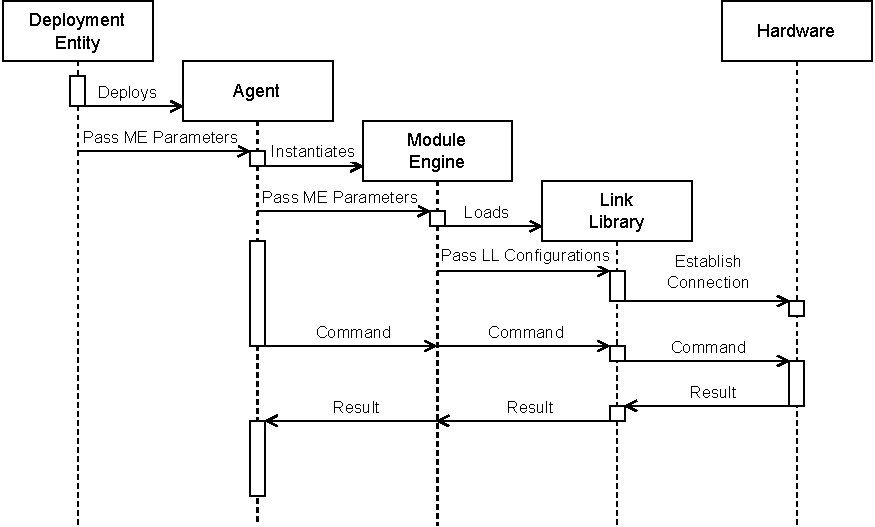
\includegraphics[scale=0.85]{Module_Engine_Sequence_Diagram}
	\caption{Sequence diagram of \acrlong{ME} operations.}
	\label{fig:module_engine_sequence_diagram}
\end{figure}

The \acrshort{ME} will need a method to parse the marketplace file and extract from it the name and path to the location of the \acrshort{LL}, sorting them into a lookup table, for faster access.

It would also need a method to load a \acrlong{LL} given its type and provide the loaded \acrshort{LL} with its configurations.

Two methods to utilize the \acrshort{LL} are also needed, to execute a command and receive its result, and to stop the \acrshort{LL} and disconnect it from the hardware.

On the \acrlong{LL} side, it would need a starter method that is run when it first loads, to initialize any needed fields and establish connection to the hardware. It needs a method to run and instruction and receive its result and a method to stop operations. Both of these last methods are the ones utilized by the \acrshort{ME}.

The only messages sent between \acrshort{ME} and \acrshort{LL} are the commands the agent sends to the hardware. This interface should not change any command whatsoever, it simply serves as an interface. It is as if the agent is communicating directly to the hardware below, as illustrated in Figure~\ref{fig:cpe_internal_communications}. 

\begin{figure}[h!]
	\centering
	\includegraphics[scale=0.85]{CPE_internal_communications}
	\caption{Cyber-Physical Entity internal communications.}
	\label{fig:cpe_internal_communications}
\end{figure}

\section{Multi-Agent System}
\label{sec:multi-agent_system}

To showcase the functionalities and perform tests on the \acrlong{ME}, it was necessary to develop an Industrial \acrfull{MAS}. This \acrlong{CPPS} is composed of three main types of cyber-physical entities, with two other entities performing more of a management role, used for agent deployment. The two management entities are not considered cyber-physical entities because they do not have a physical counterpart and therefore do not use the \acrshort{ME}.\\

The developed entities are:
\begin{itemize}
	\item The \acrfull{RA}, that represents any kind of physical component capable of performing processes, like a robotic arm or a bottle filling station;
	\item The \acrfull{TA}, that represent any kind of physical component capable of transporting products from one location on the shop floor to another, components like a conveyor belt or a \acrfull{AGV};
	\item The \acrfull{PA}, that represent any kind of product to be manufactured by the Industrial \acrshort{MAS};
	\item The \acrfull{DA}, that will launch \acrshortpl{RA} and \acrshortpl{TA} and provide them with the necessary parameters. This is the entity seen in Figure~\ref{fig:component_diagram};
	\item And the \acrfull{PM}, that will launch \acrshortpl{PA} and provide them with their production sequence.
\end{itemize}


When the system is first launched, the agents that start up immediately are the \acrfull{DA} and \acrfull{PM}, since both of these agents are responsible for the launch and management of all other agents. Both of them need to be capable of receiving input from a human user through a \acrfull{GUI}. The user creates the necessary agents through the \acrshort{DA} by providing it with the \acrshort{LL} type and configuration file. The \acrshort{DA} is capable of launching both \acrshortpl{RA} and \acrshortpl{TA} because these are the agents that need the \acrlong{ME} to operate as mentioned previously. Figure~\ref{fig:da_activity_diagrams} presents the process of deploying a new agent (\ref{fig:da_activity_diagram_deploy_agent}) and stopping a pre-existing agent (\ref{fig:da_activity_diagram_stop_agent}). The marketplace file is not provided by the user, but could instead be provided by some kind of web application. For this work however, it is provided locally and the \acrshort{DA} has access to its contents directly.\\

\begin{figure}[h!]
	\centering
	\subbottom[Deployment of new agent.\label{fig:da_activity_diagram_deploy_agent}]{%
		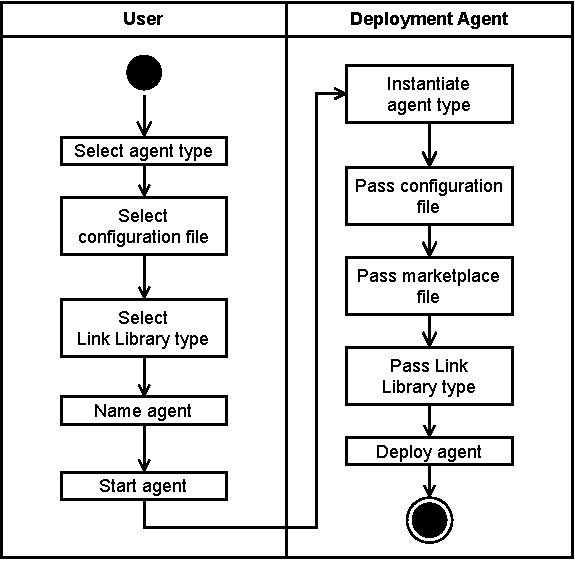
\includegraphics[width=0.47\linewidth]{Activity_Diagram_DA_deploy}}%
	\hspace{0.40cm}
	\subbottom[Termination of running agent.\label{fig:da_activity_diagram_stop_agent}]{%
		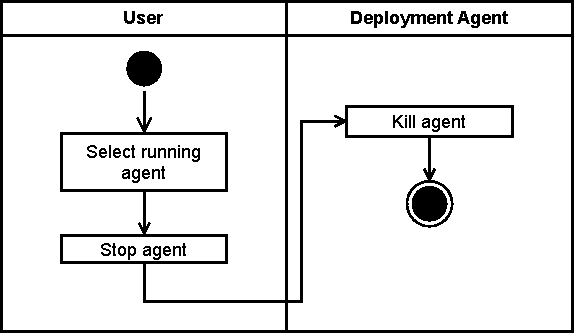
\includegraphics[width=0.47\linewidth]{Activity_Diagram_DA_stop}}%
	\caption{\acrlong{DA} activity diagram.}
	\label{fig:da_activity_diagrams}
\end{figure}

The \acrlong{PM} is simpler in its activities, since its only task is to launch \acrlongpl{PA}. A user only has to start the agent through the \acrshort{GUI} of the \acrshort{PM}. When a \acrshort{PA} is started, it does not need any other external parameters. Figure~\ref{fig:pm_activity_diagram} presents this simple operation. Since the \acrshort{PM} does not terminate the \acrshortpl{PA}, it only has the functionality to deploy agents.\\

\begin{figure}[h!]
	\centering
	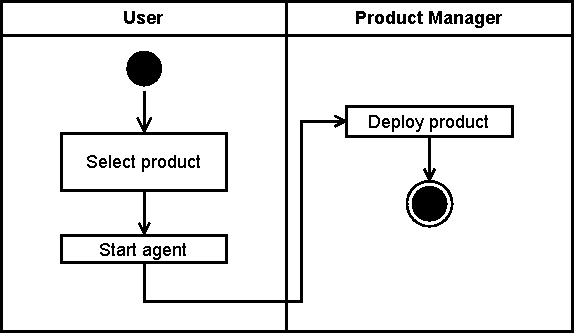
\includegraphics[scale=0.9]{Activity_Diagram_PM}
	\caption{\acrlong{PM} activity diagram.}
	\label{fig:pm_activity_diagram}
\end{figure}

After deployment, \acrlongpl{RA} and \acrlongpl{TA} will instantiate the \acrlong{ME} and pass it the marketplace and configuration files, along with the \acrshort{LL} type. Then they will proceed to register themselves in a Yellow Pages Service, which is a way for agents to search for other agents with specific characteristics. This service works a little bit like a phone book, presenting all registered agents along with their agent ID, a unique identifier that corresponds to each agent. Any agent can access the Yellow Pages and search for agents with certain capabilities, called skills. These skills show what actions an agent can perform. For example, an agent with a skill called "Move\_to\_Storage" might move itself or a load to storage, or an agent with the skill "Staple\_tag" might be able to staple a tag on a piece of clothing, and so on. A production sequence is list of the skills a product needs to be performed in order to complete it fabricated. In the designed system, \acrlongpl{PA} can use the Yellow Pages to look for \acrshortpl{RA} and \acrshortpl{TA} capable of performing the needed skills.\\

When all \acrshortpl{RA} and \acrshortpl{TA} have been launched and their initial setup completed, the system is now ready to work. \acrshortpl{PA} are launched as new products enter the production line, and after getting their production sequences, they will search the Yellow Pages to find a \acrshort{RA} capable of performing the first skill. When they find it, they will issue a Call for Proposals from all relevant agents through the \acrshort{FIPA} Contract Net. This interaction protocol was developed by \acrshort{FIPA}, and it works as follows:

In this protocol the agent that starts the communication is called the Initiator, and all other are the Participants. The Initiator sends a Call for Proposals or CFP message to all Participants preselected by the Initiator. After receiving the message, the Participants can either accept the call by sending a Proposal, or refuse altogether. On refusal, this particular Participant is out of communications from now on. Proposals might include some data to help the Initiator decide which Participants it wants to keep communicating with. Upon deciding this, the Initiator will send an Accept Proposal message to the desired Participants, Rejecting all other Proposals. Finally, the Participants whose Proposal was accepted might perform some process and inform the Initiator of the result, with a Failure message or a Inform message. This interaction protocol can be visualized in Figure~\ref{fig:contract_net_protocol}.\\

\begin{figure}[h!]
	\centering
	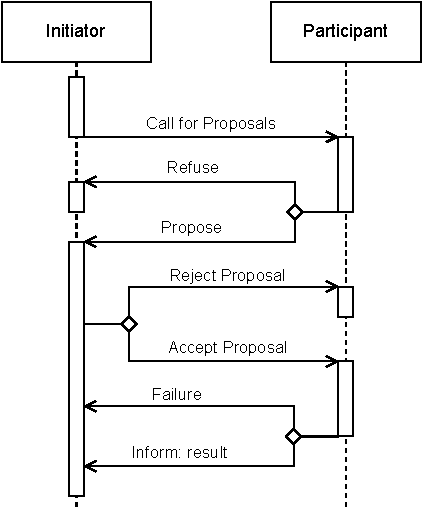
\includegraphics[scale=0.87]{FIPA_Contract_Net}
	\caption{\acrshort{FIPA} Contract Net interaction protocol. Adapted from \cite{FIPA_Contract_Net}.}
	\label{fig:contract_net_protocol}
\end{figure}

After receiving the Call for Proposals, \acrshortpl{RA} will respond with a Proposal. This simply signifies that the agent is available to perform the needed skill, and it does not contain any extra data. Then the \acrshort{PA}, the Initiator, will Accept the first Proposal on the responses list for simplicity. Finally the selected \acrshort{RA} will respond with an Inform message, in which the contents of the message contain the location of the \acrshort{RA} on the shop floor. This location will be used by the \acrshort{PA} to ask for transportation from a \acrshort{TA}. An example of a communication through the \acrshort{FIPA} Contract Net can be seen in Figure~\ref{fig:pa_ra_contract_net}. In this example, two \acrshortpl{RA} have the relevant skill for the \acrshort{PA}. It selects the first one and rejects the other. Then the \acrshort{RA} Informs the \acrshort{PA} of their location.\\

\begin{figure}[h!]
	\centering
	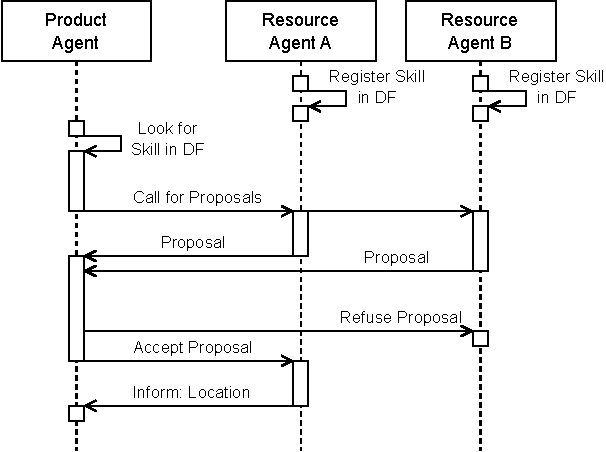
\includegraphics{PA_RA_Contract_Net}
	\caption{\acrshort{FIPA} Contract Net protocol between a \acrlong{PA} and two \acrlongpl{RA}.}
	\label{fig:pa_ra_contract_net}
\end{figure}

Upon finding a \acrlong{RA}, the \acrlong{PA} now needs to be transported to its work station. For this it needs a \acrlong{TA}. So the \acrshort{PA} will once again look into the Yellow Pages for a \acrshort{TA}, by searching for a skill once again. It was decided that for simplicity, only one transport agent will be used in the simulated system. So instead of asking for an agent through the \acrshort{FIPA} Contract Net, the agent can skip straight away to the next step, which is to ask for a skill to be performed through a \acrshort{FIPA} Request. This protocol is also one created by \acrshort{FIPA}, and its less complex than the \acrshort{FIPA} Contract Net:

This protocol also includes an Initiator, but only one Participant. This is a one to one communication. The Initiator starts by sending a Request to the Participant. At this point the Participant may Refuse, and communications are terminated. If it Agrees however, it will start performing the desired process immediately. Upon completion, it will notify the Initiator with either a Failure or Inform message. This protocol is shown in Figure~\ref{fig:requests_protocol}.\\

\begin{figure}[h!]
	\centering
	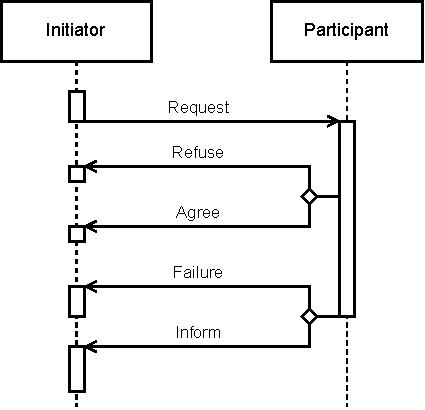
\includegraphics{FIPA_Requests}
	\caption{\acrshort{FIPA} Request interaction protocol. Adapted from \cite{FIPA_Request}.}
	\label{fig:requests_protocol}
\end{figure}

The \acrshort{PA} starts a \acrshort{FIPA} Request with its starting and ending positions, so the \acrshort{TA} from where the \acrshort{PA} departs from, and what is its destination. After Agreeing with the Request and before the communication terminates, the \acrshort{TA} will transport the \acrshort{PA} to the destination and send an Inform message signalling the transportation is complete. After arriving at the location where the previously found \acrshort{RA} is located, the \acrshort{PA} will use the same protocol to Request the skill from the \acrshort{RA}. Both of these sequences of messages are shown in Figure~\ref{fig:agent_requests}. In \ref{fig:pa_ra_requests} the \acrshort{FIPA} Requests protocol between a \acrshort{PA} and \acrshort{TA} is shown, and in \ref{fig:pa_ta_requests} between a \acrshort{PA} and \acrshort{RA}.\\

\begin{figure}[h!]
	\centering
	\subbottom[\acrlong{PA} and \acrlong{TA}.\label{fig:pa_ra_requests}]{%
		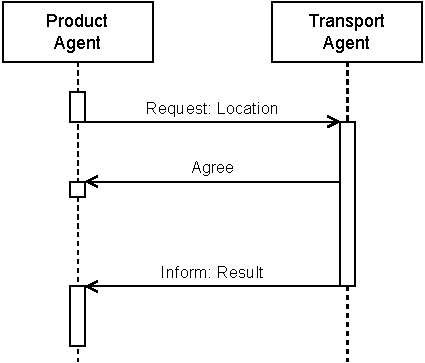
\includegraphics[width=0.45\linewidth]{PA_TA_Requests}}%
	\hspace{0.55cm}
	\subbottom[\acrlong{PA} and \acrlong{RA}.\label{fig:pa_ta_requests}]{%
		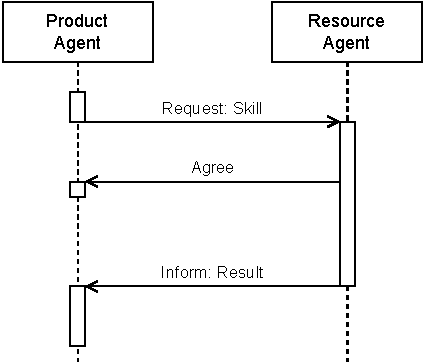
\includegraphics[width=0.45\linewidth]{PA_RA_Requests}}%
	\caption{\acrshort{FIPA} Requests between agents.}
	\label{fig:agent_requests}
\end{figure}

When the \acrshort{RA} finishes it skill and informs the \acrshort{PA}, the \acrshort{PA} will check if its production sequence is complete. If it is, it will Request transportation from a \acrshort{TA} to storage. If the sequence is not complete, it restarts the process by checking the Yellow Pages for agents capable of performing the next skill, Calling for Proposals, and so on. The whole evolution of the \acrshort{MAS} can be visualized in Figure~\ref{fig:mas_activity_diagram}. It only shows the full interactions between agents, their actions and decisions without the \acrlong{ME}.\\

\begin{figure}[h!]
	\centering
	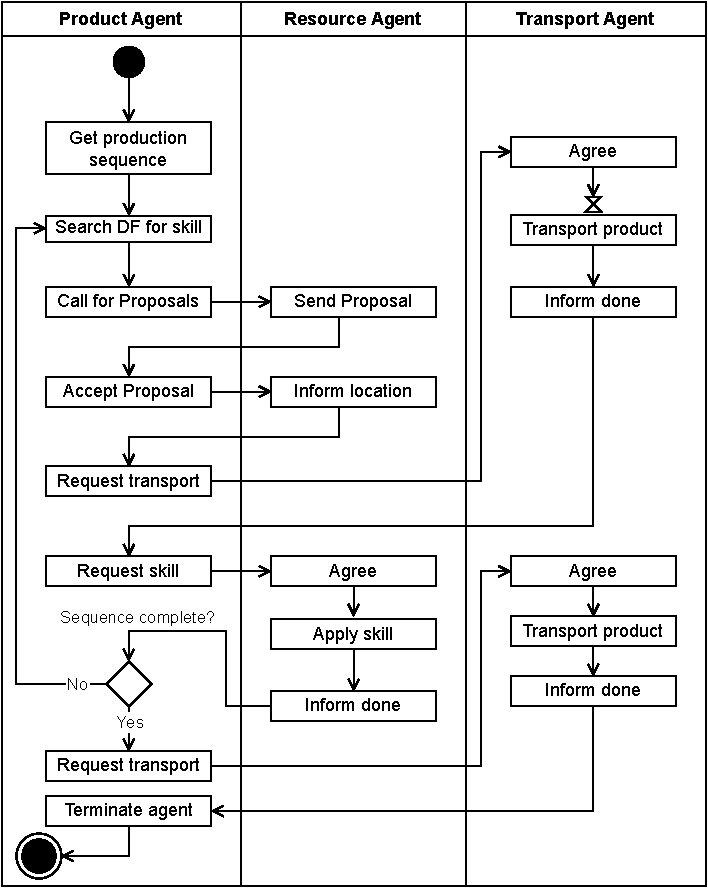
\includegraphics{MAS_Activity_Diagram}
	\caption{Activity diagram of the Industrial \acrlong{MAS}.}
	\label{fig:mas_activity_diagram}
\end{figure}

\section{System Overview}
\label{sec:system_overview}

Now that all parts of the system have been explained, it is now time to do a brief overview of the behaviour of the system has a whole. When the \acrshort{MAS} is launched, the first two agents that start up immediately are the \acrlong{DA} and the \acrlong{PM}. Then a user needs to launch the \acrlongpl{RA} and the \acrlong{TA} and select the right configurations for each agent.\\ 

When these agents are launched, they will register themselves in the Yellow Pages Service with their skills and instantiate their \acrlong{ME}, which will in turn load the corresponding \acrlong{LL}. These \acrshortpl{LL} will establish connection to the hardware. After all of these agents are deployed and ready to operate, the user can now launch the \acrlong{PA}.\\

Upon being launched, the \acrshort{PA} will look at the Yellow Pages and it will find the \acrshortpl{RA} capable of performing the first skill in its production sequence. Then it will establish contact with all of them through the \acrshort{FIPA} Contract Net. After receiving the Proposals, it will select one and refuse the all others. In the last message, the \acrshort{PA} will receive the location of the station where the \acrshort{RA} is located.\\

The next step is to Request transportation from a \acrshort{TA} to this location. The \acrshort{PA} will start a \acrshort{FIPA} Request with its current location and its destination. The \acrshort{TA} will answer this Request to signal it received the message and will immediately start the process of moving the product. For this, it will send the command through the \acrlong{ME} and through the \acrlong{LL}, to the hardware. Once the hardware finishes executing it, it will return the result back up through the \acrshort{LL} and through the \acrshort{ME} to the agent.\\

The \acrshort{TA} will now notify the \acrshort{PA} that transportation is complete. The \acrshort{PA} then starts another \acrshort{FIPA} Request, this time to the previously chosen \acrshort{RA}. This agent will execute its skill by using the same process as the \acrshort{TA}. Through the \acrshort{ME} and \acrshort{LL} down to the hardware. After the result arrives back at the agent, it will notify the \acrshort{PA}. If this is the last skill in this products production sequence, the \acrshort{PA} will now Request another transportation, but this time to storage, terminating the agent and ending its production. If, however, there are still skills in the production sequence, then the process restarts. The \acrshort{PA} will search again for a \acrshort{PA} capable of performing the new skill in the sequence and so on. In Figure~\ref{fig:complete_activity_diagram}, this whole process is shown, from start to finish.\\

\begin{figure}[h!]
	\centering
	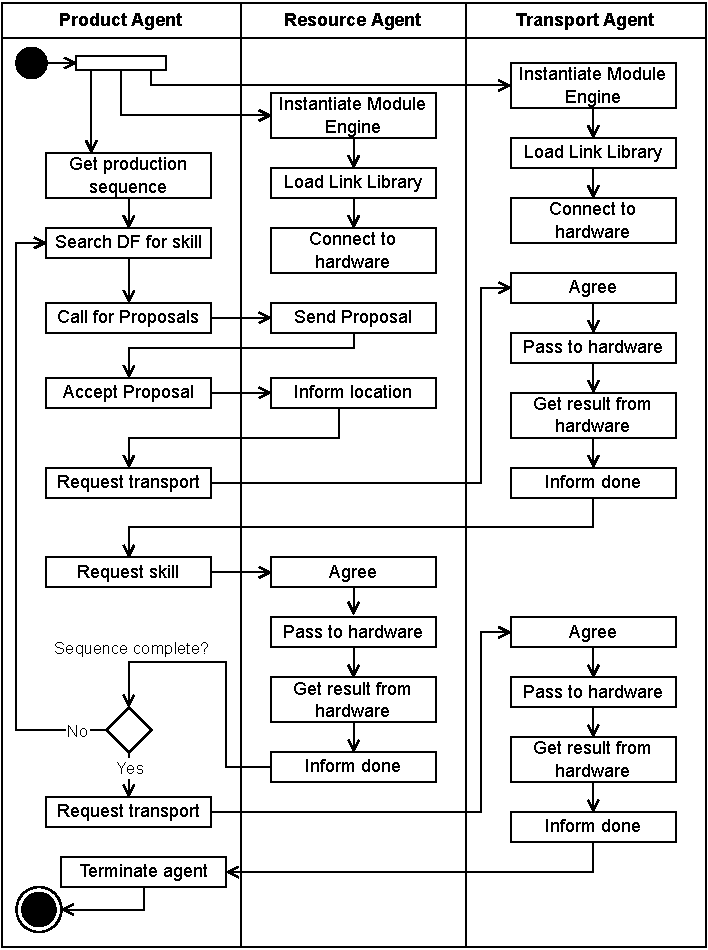
\includegraphics{Complete_System_Activity_Diagram}
	\caption{Activity diagram of the final system.}
	\label{fig:complete_activity_diagram}
\end{figure}
